\chapter{Knihovna publicvfk}
\label{4-plugin}
Tato kapitola bude věnována informacím o nové knihovně \textbf{publicvfk} pro zásuvný modul \textit{QGIS VFK Plugin} a její implementaci. Uvedu zde co je pro knihovnu vstupem a co výstupem. Dále uvedu ukázky funkčnosti na testovacích datech a doplním informace o způsobu implementace do výše zmíněného zásuvného moudlu. Pro tvorbu jsem čerpal z těchto zdrojů \cite{cookbook, ucebnicepython}

\section{Vstupní data}
Vstupními daty pro knihovnu je textový soubor ve formátu VFK s neúplnými daty. Knihovna přebírá adresu vstupního souboru a dochází k načtení dat a zápisu do databáze.
\section{Testovací data}
Zabalená testovací data ve formátu VFK byla stažena pro katastrální území Abertamy na adrese: \href{http://services.cuzk.cz/vfk/ku/20170901/600016.zip}{http://services.cuzk.cz/vfk/ku/20170901/600016.zip}.

\begin{figure}[H]
	 \centering
      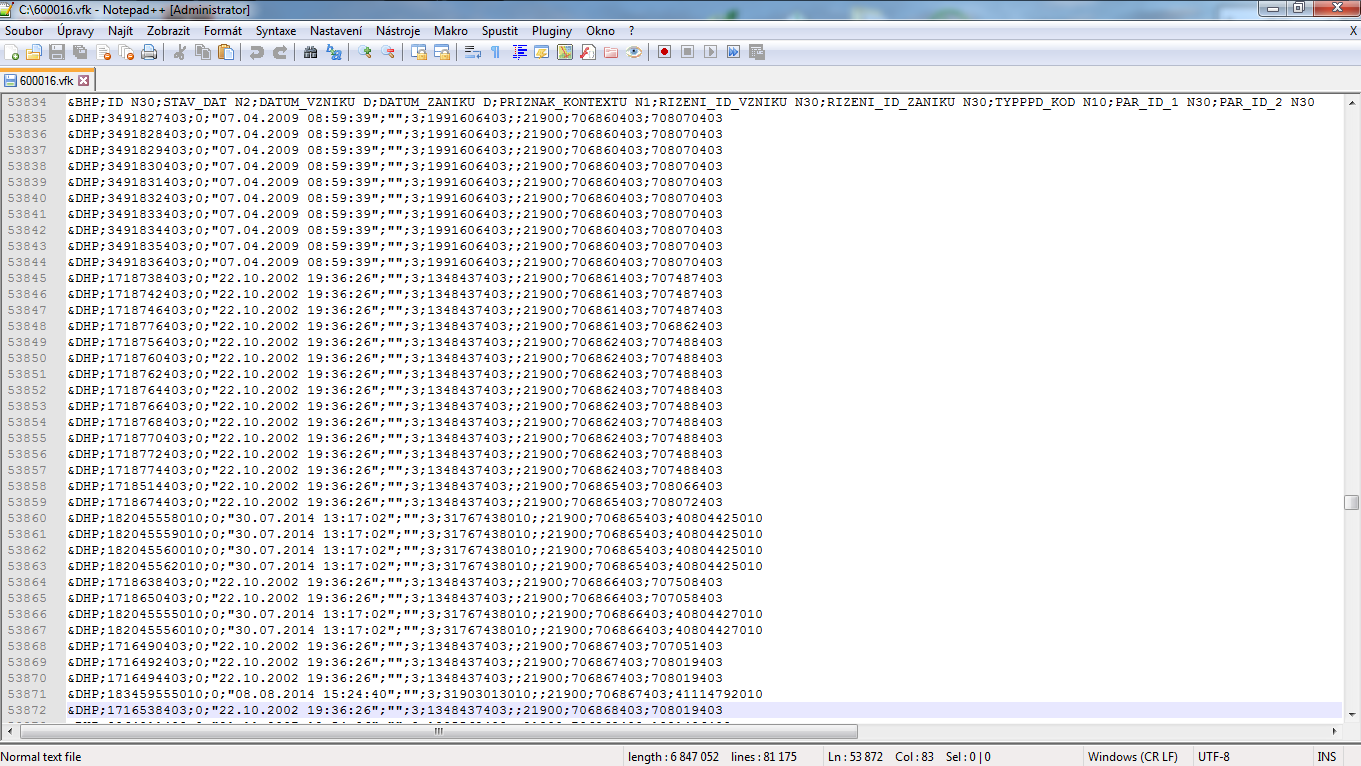
\includegraphics[width=15cm]{./pictures/testovaci_data.png}
      \caption{Ukázka bloku hranic parcel(HP) -- definice bloků a věty dat(zdroj:vlastní)}
      \label{fig:testovaci_data}
  \end{figure}
\begin{table}  
\caption{Ukázka bloku hranic parcel(HP) -- definice bloků a věty dat(zdroj:vlastní)}
\noindent\begin{tabular}{|p{\textwidth}|}
    \hline
    Zkouška vysázení \_ nebo třeba \% a co takhle \& to funguje? Zkouška vysázení \_ nebo třeba \% a co takhle \& to funguje? Zkouška vysázení \_ nebo třeba \% a co takhle \& to funguje?  \\ \hline
    Tak tohle už vypadá lépe: \_ nebo třeba \% \\ \hline
    kmenove\_cislo\_par \\ \hline
    \hline 
    \end{tabular}
\end{table}

\section{Výstupní data}
Výstupem k knihovny je sestavená geometrie pro bloky parcel a budov. Geometrie je společně s dalšími hodnotami jako je identifikační číslo, číslo parcely zapsána do vytvořené databáze.
\section{Popis tříd knihovny a jejich metod}
V této podkapitole představím jednotlivé třídy knihovny a jejich členské metody. Popíši, co která třída a metoda obstarává.
\subsection{VFKParBuillderError}
Tato třída dědí vlastnosti třídy Exception a je volána v případě že nastane chyba. To se může stát v případě nepřipojeného \zk{VFK} souboru nebo databáze.
%\subsection{VFKBuillder}
%\subsection{VFKBudBuillder}
\subsection{VFKParBuillder}
V této třídě dochází k samotnému sestavení geometrie parcel, vytvoření nové tabulky PAR v databázi a zapsání. Zapisuje se identifikační číslo parcely(\verb|par_id|), kmenové číslo parcely(\verb|kmenove_cislo_par|), poddělení čísla parcely(\verb|poddeleni_cisla_par|) a samozřejmě geometrie dané parcely. Zápis do databáze je proveden transakcí, čímž je zaručené zapsání všech parcel nebo žádné - v případě chyby.

\begin{itemize}
\item \verb|__init__(self,filename)|
		
Konstruktor třídy, má jeden parametr - cestu k VFK souboru. Dochází zde k vytvoření tabulky geometrie (\verb|geometry columns|) a tabulky souřadného systému (\verb|spatial_ref_sys|) bez kterých by nebylo možné číst geometrii z databáze. V případě nepřipojeného zdroje dat - vfk souboru, je volána třída VFKParBuilderError.
\item \verb|get_par(self)|
		
Tato metoda vrací seznam unikátních identifikačních čísel parcel, který získá SQL dotazem, ve formátu seznamu. Opět je volána třída VFKParBuilderError v případě nepřipojené databáze.
\item \verb|filter_hp(self, id_par)|

Na základě identifikačního čísla parcely najde všechny hranice, které k dané parcele patří a vrací je uložené v seznamu. Volána třída VFKParBuilderError v případě nepřipojené databáze.
\item \verb|build_par(self, list_hp)|

Jedna z hlavních metod, která sestavuje geometrii jednotlivých parcel a ukládá jí do ringu. Parametrem je seznam hranic dané parcely. V případě parcely s dírami si vytvoří seznam ringů, ve kterém na závěr najde největší ohraničující ring a ze zbylých ringů udělá díry. Sestavení probíhá geometrickou cestou. Nejdříve je přidána první hranice, poté hranice co má začíná koncovým bodem první hranice a tak dokola.
\item \verb|add_boundary(self,position,direction, list_hp, ring)|

Metoda pro přidávání jedné hranice do ringu. Jako parametr dostává pozici dané hranice v seznamu, aby mohla být hranice ze seznamu odstraněna. Dále směr orientace přidávané hranice - všechny hranice nemají stejnou orientaci. Některé navazují na koncový bod koncovým, tudíž je potřeba body hranice přidávat "odzadu". Poslední dva parametry jsou ring, do kterého hranici přidává a seznam hranic parcely, ze kterého hranici vezme a odstraní. 
\item \verb|build_all(self, limit=None)|

Zde probíhá samotné sestavení všech parcel. Po sestavení je parcela uložena do databáze. Ukládání parcel je zabaleno do transakce. Metodě je možné nastavit limit kolik parcel má sestavit přes parametr limit, který je základně nastaven na hodnotu None.
\item \verb|get_sql_commands_from_file(self, fileName)|

Metoda otevírající soubor a vracející seznam SQL příkazů. Jediným parametrem je cesta k souboru.
\item \verb|add_tables(self, sqlfileName)|

Provádí příkazy, které dostane z metody \verb|get_sql_commands_from_file(self, fileName)|. Cesta k souboru s příkazy je jediným parametrem. Po ukončení cyklu s SQL příkazy je třeba zavolat metodu \textit{commit()} jinak nedojde z provedení posledního příkazu. Důvode je ten, že provádění příkazů probíhá interně v transakci, kterou je třeba pro správné provedení ukončit.
\end{itemize}
\section{Implementace knihovny}
Základem implementace bylo správné umístění do kódu zásuvného modulu. Potřeboval jsem zachovat funkcionalitu při otevření úplných i neúplných dat. Jsou-li data úplná, funguje zásuvný modul standardně. Pokud data neobsahují bloky PAR a BUD -- jsou neúplná, dojde k jejich sestavení a tedy zavolání třídy z nově implementované knihovny.